\documentclass{gost7.32-2001}


\subject{Длинное название темы, которое не умещается на одной строчке, например}
\student{Фамилия Имя Отчество}
\captain{Капитан О. К.}
\inspector{Иванов А. П.}
\reviewerinfo{очень крутая должность}
\reviewer{Фамилия И. О.}
\secretary{Иванов А. П.}
\departmenthead{Зефиров С. Л.}

\begin{document}
\maketitle

\anonsection{Реферат}

\info

ТЕЛЕКОММУНИКАЦИОННАЯ СИСТЕМА, ИНФОЛОГИЧЕСКАЯ МОДЕЛЬ, СТРУКТУРНАЯ МОДЕЛЬ, ФИЗИЧЕСКАЯ МОДЕЛЬ, ТОПОЛОГИЯ СЕТИ.

Объектом исследования являются телекоммуникационные системы организаций и обеспечение их безопасности.

Целью курсового проекта является проектирование телекоммуникационной системы для организации и оценка стоимости ее создания. 

В процессе работы были созданы инфологическая, структурная и физическая модели телекоммуникационной системы для торгового склада. Разработана схема адресации и проведена стоимостная оценка. Построена модель телекоммункационной системы в среде Cisco Packet Tracer.

\newpage
\tableofcontents
\specsection{Введение}
Телекоммуникационные системы  присутствуют в большинстве современных организаций. Грамотное проектирование телекоммуникационных систем является важнейшим  аспектом работы специалиста в области информационной безопасности. 

Актуальность курсовой работы состоит в обеспечении защиты от несанкционированного доступа к оборудованию, входящему в телекоммуникационную систему, устойчивости к внешним воздействиям и оправданности ее использования в организации с финансовой точки зрения.

Первый этап курсового проекта состоит в составлении инфологической модели локальной телекоммуникационной системы организации.

Второй этап \hyp{} создание структурной схемы локальной телекоммуникационной системы организации.

Третий этап \hyp{} создание физической модели кабельной подсистемы локальной телекоммуникационной системы организации.

Четвертый этап \hyp{} создание схемы адресации узлов локальной телекоммуникационной системы.

Пятый этап \hyp{} создание модели телекоммуникационной системы в среде Cisco Packet Tracer.
\newpage
\section{Раздел1}
\eqref{eq:1}
\subsection{Подраздел1}
\paragraph{Пункт с заголовком1}
В приложении \ref{prove2} текст, текст, текст, текст, текст, текст, текст, текст, текст, текст, текст, текст, текст, текст
\paragraph{Пункт с заголовком2}
\subparagraph Подпункт текст, текст, текст, текст, текст, текст, текст, текст, текст, текст, текст, текст, текст, текст
\subparagraph Подпункт  текст, текст, текст, текст, текст, текст, текст, текст, текст, текст, текст, текст, текст, текст

sdojfh aslsakjf sadlkf sadfl sdfjh fsdalk
\begin{enumerate}
\item one;
\item two;
\item three;
  \begin{enumerate}
  \item one;
  \item two;
  \item three;
  \end{enumerate}
\end{enumerate}

\begin{equation}
  y = sin(x)
\end{equation}

\begin{equation}
  y = sin(x)
\end{equation}

\begin{equation}
  y = sin(x)
\end{equation}

\begin{equation}
  y = sin(x)
\end{equation}
\subsection{Подраздел2}
\paragraph{Пункт с заголовком1}
Текст, текст, текст, текст, текст, текст, текст, текст, текст, текст, текст, текст, текст, текст

\begin{equation}
  y = sin(x)
\end{equation}

\begin{equation}
  y = sin(x)
\end{equation}
\section{Раздел2}
\paragraph{Пункт с заголовком 1} Текст, текст, текст, текст, текст, текст, текст, текст, текст, текст, текст, текст, текст, текст
\paragraph{}Пункт без заголовка текст, текст, текст, текст, текст, текст, текст, текст, текст, текст, текст, текст, текст, текст  \cite{ltks, asd}.
\begin{itemize}
\item one;
\item two;
\item three;
  \begin{itemize}
  \item one;
  \item two;
  \item three;
  \end{itemize}
\end{itemize}

\begin{equation}
  y = sin(x)
\end{equation}

\begin{equation}
  y = sin(x)
\end{equation}

% \section{Инфологическая модель локальной телекоммуникационной системы организации}
\label{sec:inf_model}
В ходе выполнения задания требовалось определить бизнес-цель организациии. Бизнес-целью торгового склада является предоставление потребителям необходимых строительных материалов.

Для достижения этой цели торговый склад выполняет следующие функции:
\begin{itemize}
\item прием товара от поставщиков;
\item учет товара;
\item выдачу товара покупателям;
\item подготовление отчетности;
\item передача информации продавцу наличии/отсутствии товара.
\end{itemize}


Для ТКС торгового склада целевой функцией может являться автоматизация учета товара. ТКС может быть задействована в следующих процессах:
\begin{itemize}
\item контроль операций с товаром;
\item установление кантакта с поставщиками;
\item предоставление доступа к сайту/БД;
\item печать документов;
\item составление и отправка отчетности в контроллирующие органы.
\end{itemize}


Была проведена декомпозиция целевой функции системы для детального описания процессов, необходимых для ее выполнения. Описание процессов проведено с помощью методологии функционального моделирования IDEF0. Результат выполнения декомпозиции приведен на рисунках \ref{fig:idef0-common} и \ref{fig:idef0-inside}.

\begin{sidewaysfigure}[!htp]
  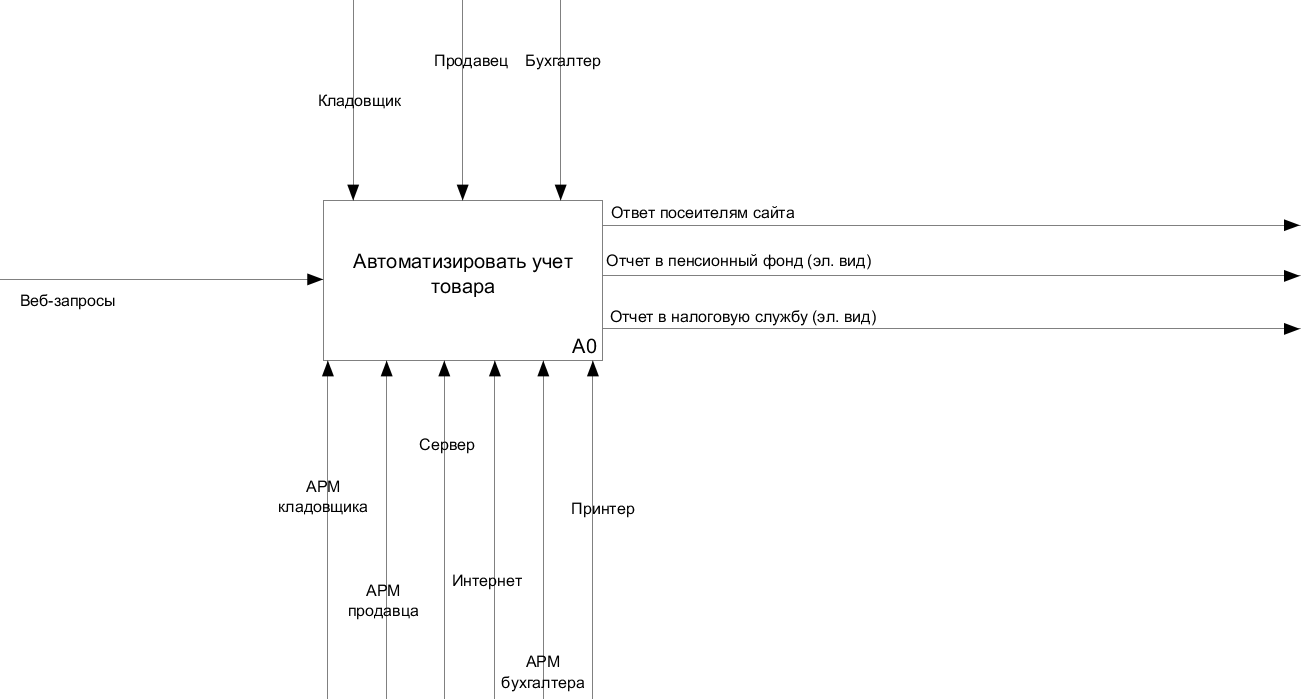
\includegraphics[width=\linewidth]{appendix/a0.png}
  \caption{Целевая функция телекоммуникационной системы торгового склада}
  \label{fig:idef0-common}
\end{sidewaysfigure}
\clearpage

\begin{sidewaysfigure}[!htp]
  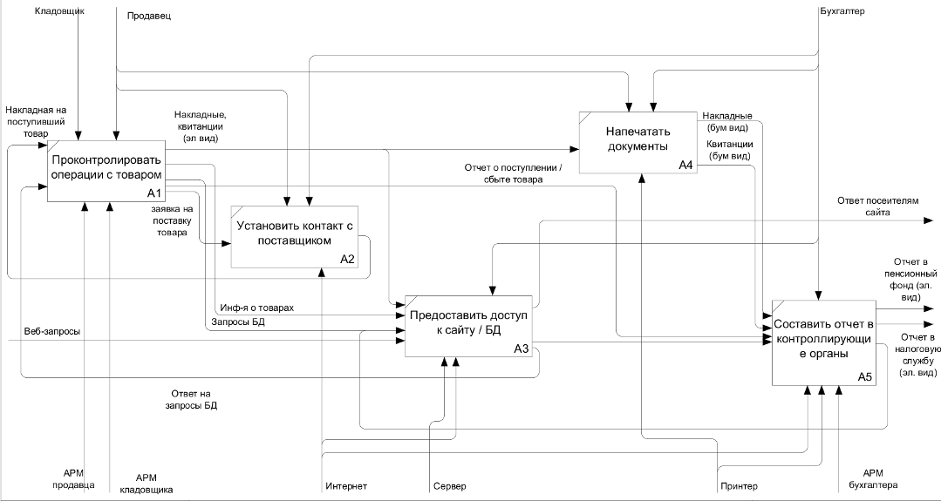
\includegraphics[width=\linewidth]{appendix/a0_2.png}
  \caption{Декомпозиция целевой функции ТКС торгового склада}
  \label{fig:idef0-inside}
\end{sidewaysfigure}
\clearpage

Графическое представление процессов приведено на рисунках \ref{fig:a1}, \ref{fig:a2}, \ref{fig:a3}, \ref{fig:a4}, \ref{fig:a5}.

\begin{figure}[H]
  \centering
  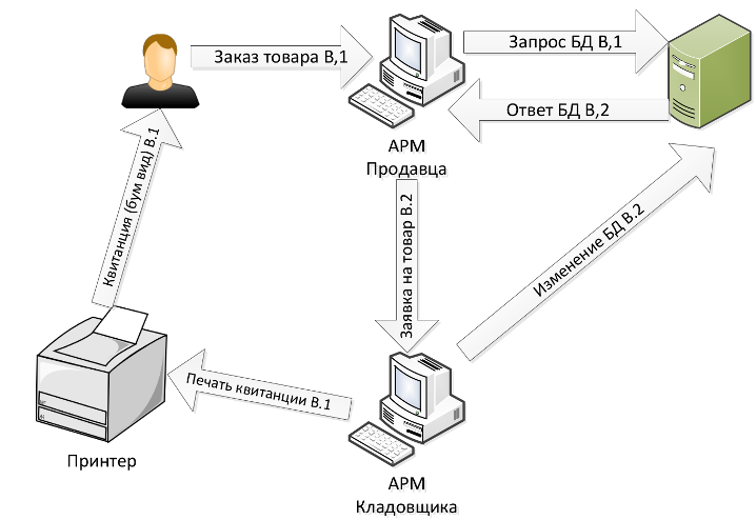
\includegraphics[width=\linewidth]{sec1/img/a1.png}
  \caption{Процесс контроля операций с товаром}
  \label{fig:a1}
\end{figure}

\begin{figure}[H]
  \centering
  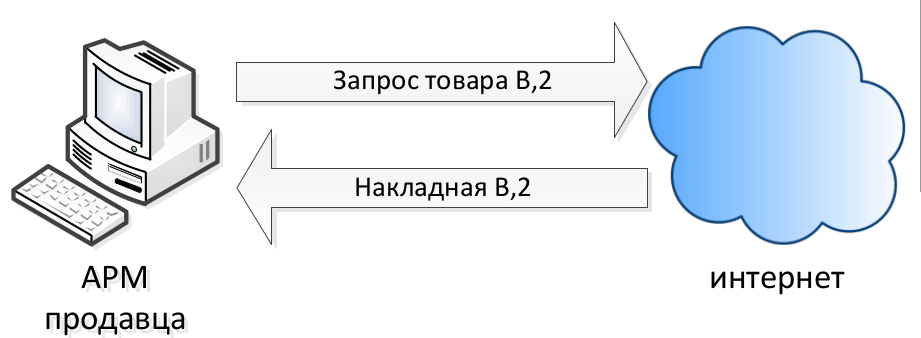
\includegraphics[width=\linewidth]{sec1/img/a2.png}
  \caption{Процесс установки контакта с поставщиком}
  \label{fig:a2}
\end{figure}

\begin{figure}[H]
  \centering
  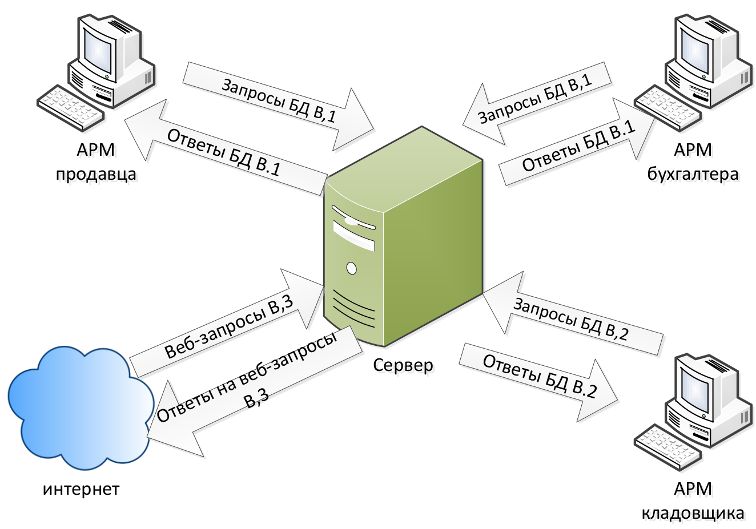
\includegraphics[width=\linewidth]{sec1/img/a3.png}
  \caption{Процесс предоставления доступа к сайту/БД}
  \label{fig:a3}
\end{figure}


\begin{figure}[H]
  \centering
  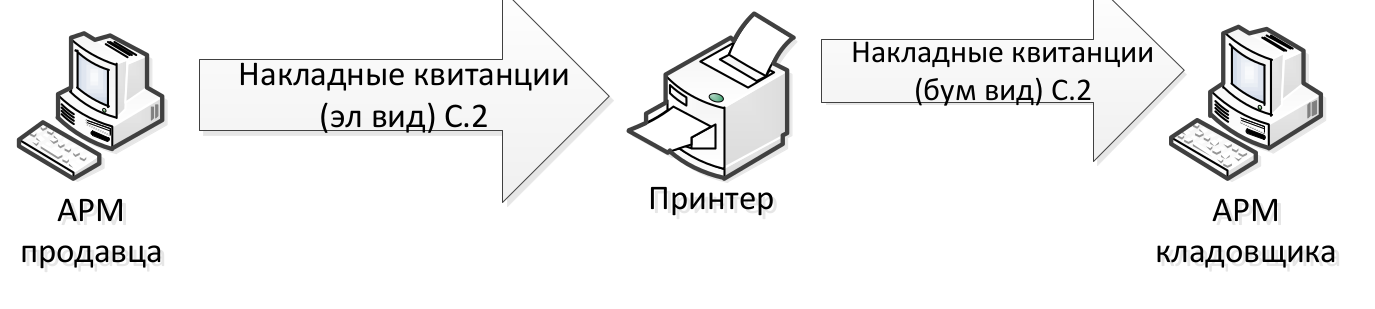
\includegraphics[width=\linewidth]{sec1/img/a4.png}
  \caption{Процесс печати документов}
  \label{fig:a4}
\end{figure}

\begin{figure}[H]
  \centering
  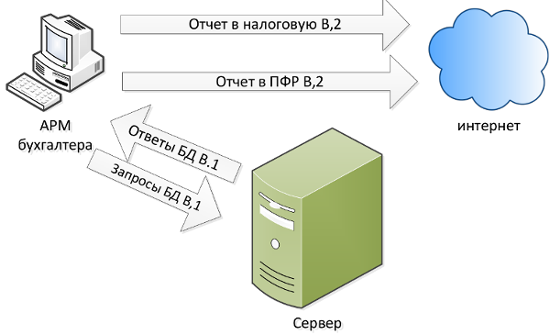
\includegraphics[width=\linewidth]{sec1/img/a5.png}
  \caption{Процесс составления и отправки отчетности}
  \label{fig:a5}
\end{figure}

Общая инфологическая модель телекоммуникационной системы торгового склада приведена на рисунке \ref{fig:total}.

\begin{figure}[H]
  \centering
  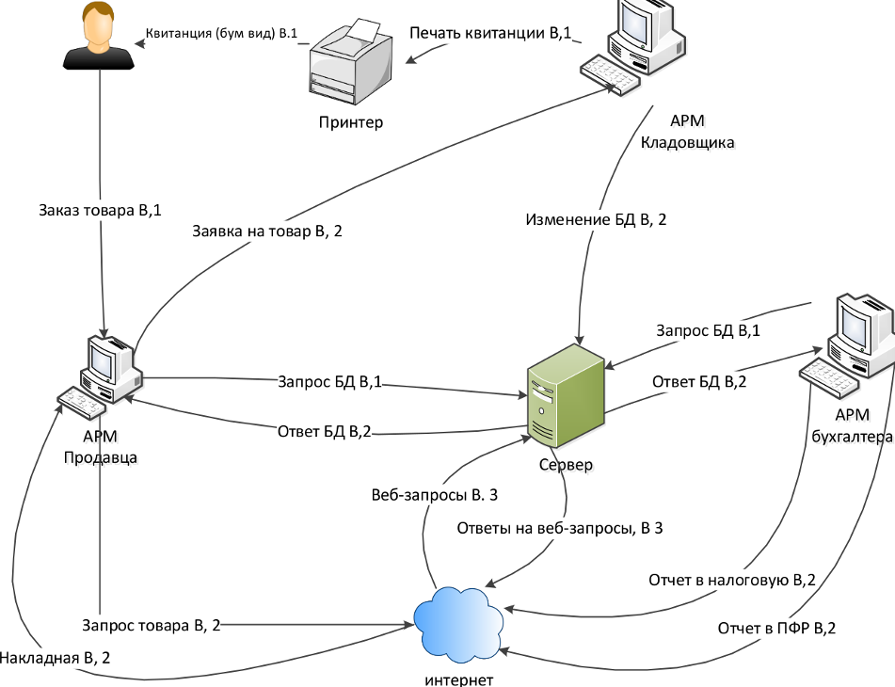
\includegraphics[width=\linewidth]{sec1/img/total.png}
  \caption{Общая инфологическая модель телекоммуникационной системы торгового склада}
  \label{fig:total}
\end{figure}


% \section{Разработка структурной модели телекоммуникационной системы торгового склада}
\label{sec:2}

Телекоммуникационная система торгового склада имеет 4 подсети:
\begin{enumerate}
\item продавцы \hyp{} 192.168.0.0/8;
\item кладовщики \hyp{} 192.168.1.0/8;
\item бухгалтер \hyp{} 192.168.2.0/8;
\item серверы \hyp{} 192.168.50.0/8.
\end{enumerate}

Данный способ деления подсетей выбран в связи с делением работников склада по должности.

Общее количество узлов сети \hyp{} 13. Подсети связаны между собой при помощи роутера. Локальная сеть сформирована при помощи технологии Ethernet. Для доступа в сеть интернет используется технология Ethernet. Данный способ доступа выбран в связи с тем, что в сети имеется сервер с сайтом.

Структурная схема представлена на рисунке \ref{fig:struct}.
\begin{figure}[H]
  \centering
  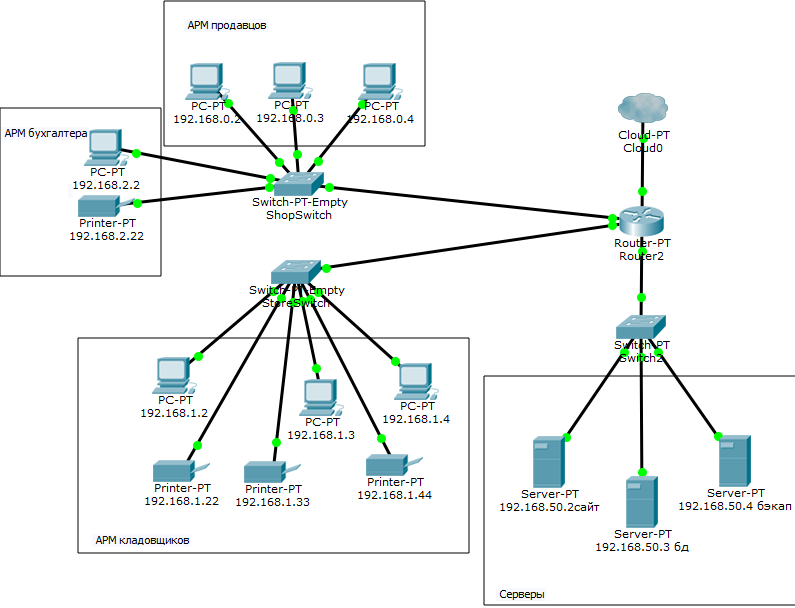
\includegraphics[width=\linewidth]{sec2/img/struct.png}
  \caption{Структурная схема телекоммуникационной системы торгового склада}
  \label{fig:struct}
\end{figure}

% \section{Проектирование физической модели телекоммуникационной системы организации}
\label{sec:3}
На основании разработанной структурной схемы организации создана физическая модель кабельной системы. При организации кабельной системы для сетей на основе проводных соединений должны учитываться различные факторы. При выборе кабеля в первую очередь учитывается требуемая длина, а также защищенность от помех и уровень собственных излучений. 

В состав торгового склада входят 2 здания: торговое и складское. Торговое здание является одноэтажным. Включает в себя 5 комнат: 3 торговых, 1 бухгалтерская и 1 серверная. Периметр здания \hyp{} 120м, площадь \hyp{} 800 $\text{м}^2$. Высота потолков \hyp{} 4 м, внешние стены кирпичные, внутренние перегородки и отделка гипсокартоновые. План торгового здания приведен на рисунке \ref{fig:shop-plane}.
\begin{figure}[H]
  \centering
  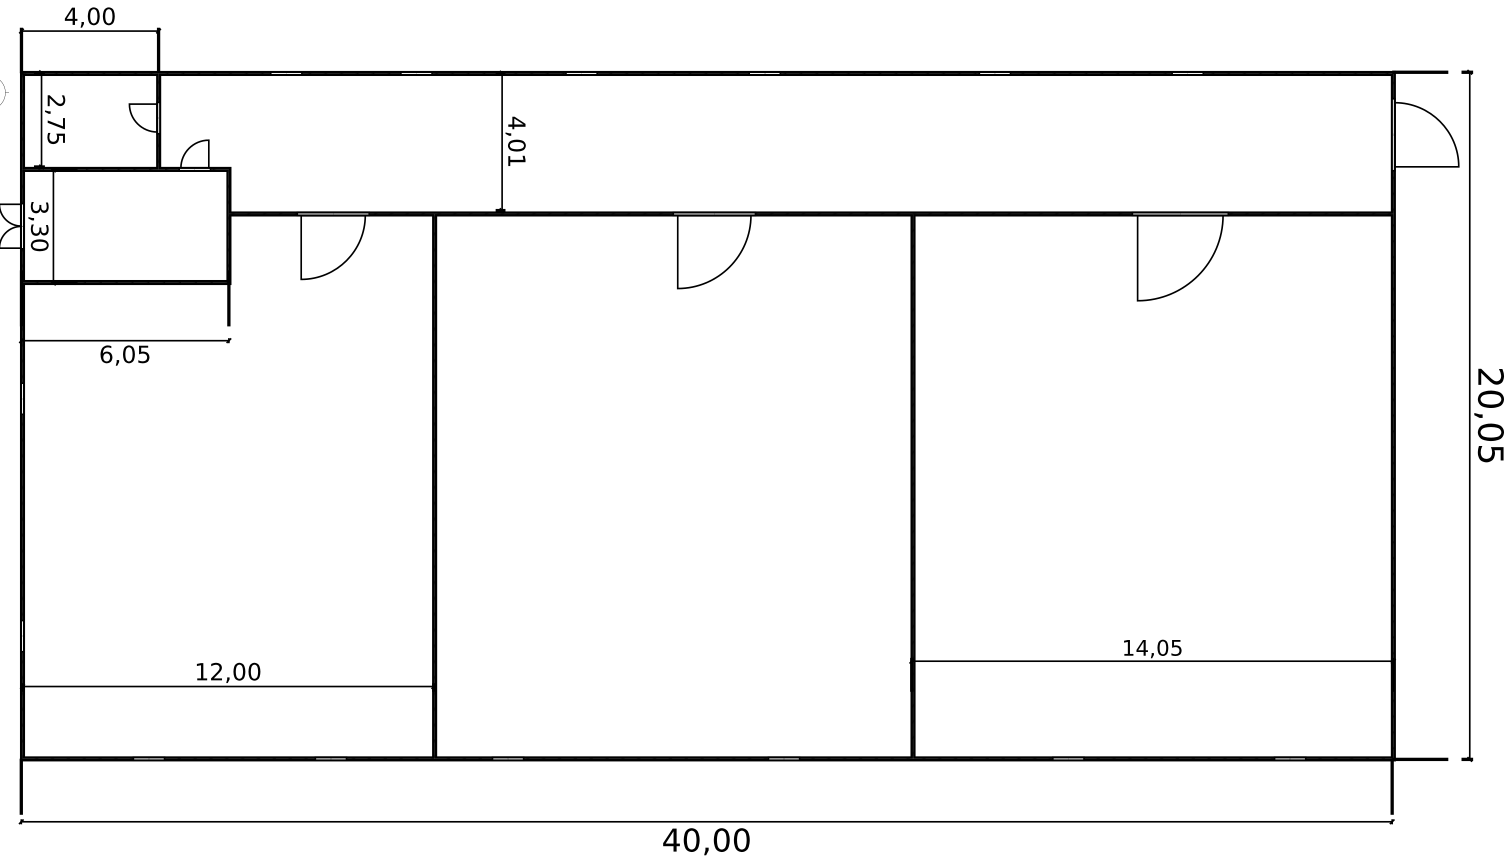
\includegraphics[width=\linewidth]{sec3/img/shop-plane.png}
  \caption{План торгового здания}
  \label{fig:shop-plane}
\end{figure}


Складское здание является одноэтажным. Включает в себя 3 складских помещения. Периметр здания 100 м, площадь \hyp{} 600 $\text{м}^2$. Высота потолков \hyp{} 6м, стены кирпичные, внутренняя отделка отсутствует. План складского здания приведен на рисунке \ref{fig:store-plane}.
\begin{figure}[H]
  \centering
  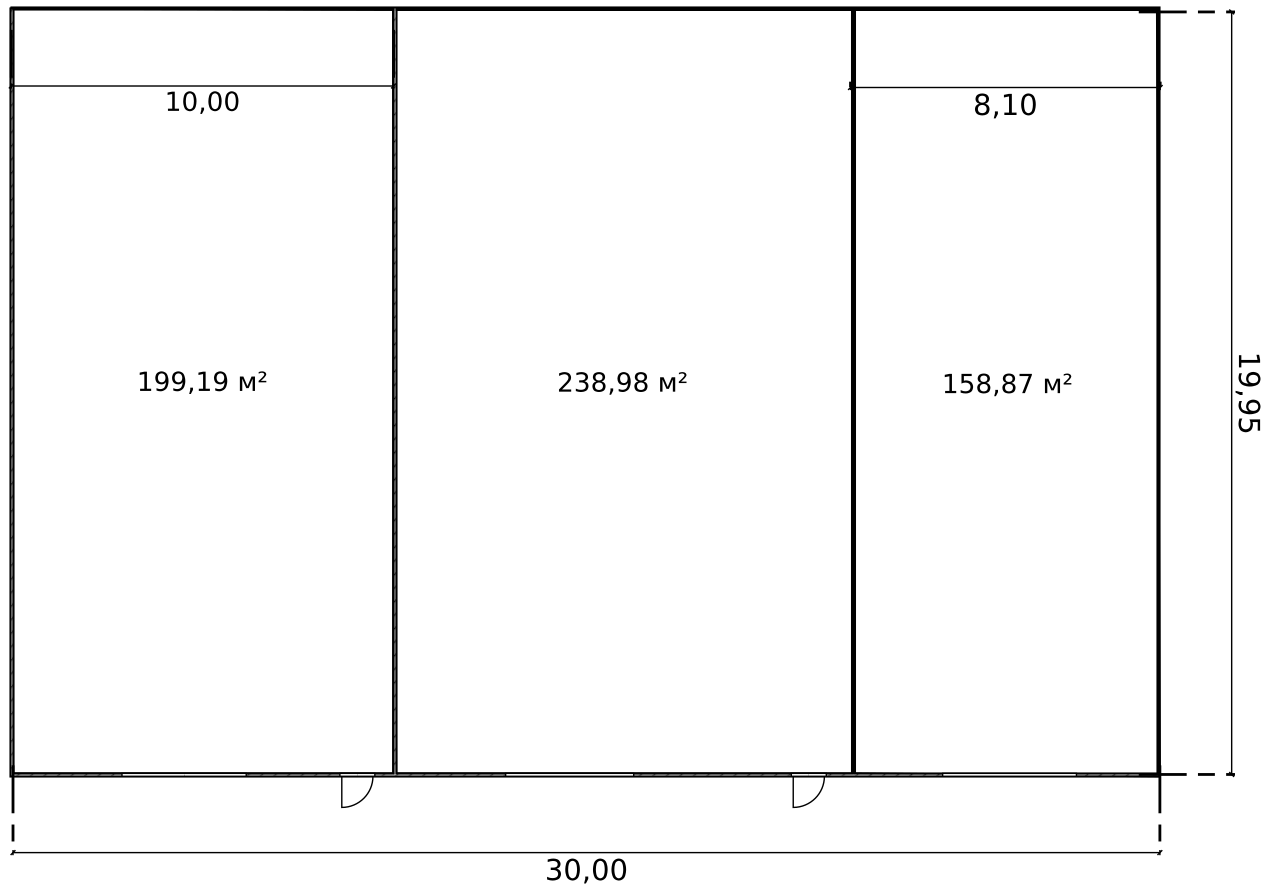
\includegraphics[width=\linewidth]{sec3/img/store-plane.png}
  \caption{План складского здания}
  \label{fig:store-plane}
\end{figure}

На планы зданий нанесено примерное расположение информационных розеток и АРМ. Результат выполнения для торгового и складского зданий приведен на рисунках \ref{fig:shop-arm} и \ref{fig:store-arm}.
\begin{figure}[H]
  \centering
  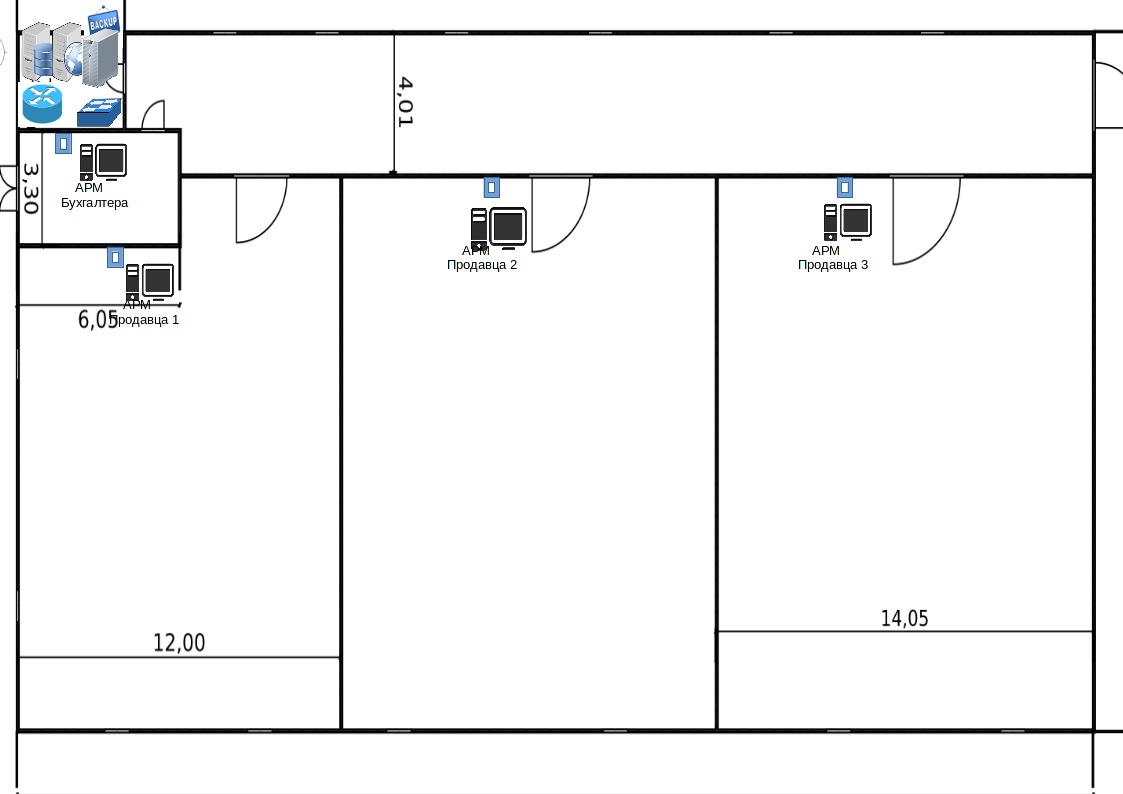
\includegraphics[width=\linewidth]{sec3/img/shop.png}
  \caption{План торгового здания с указанными положениями розеток и АРМ}
  \label{fig:shop-arm}
\end{figure}

\begin{figure}[H]
  \centering
  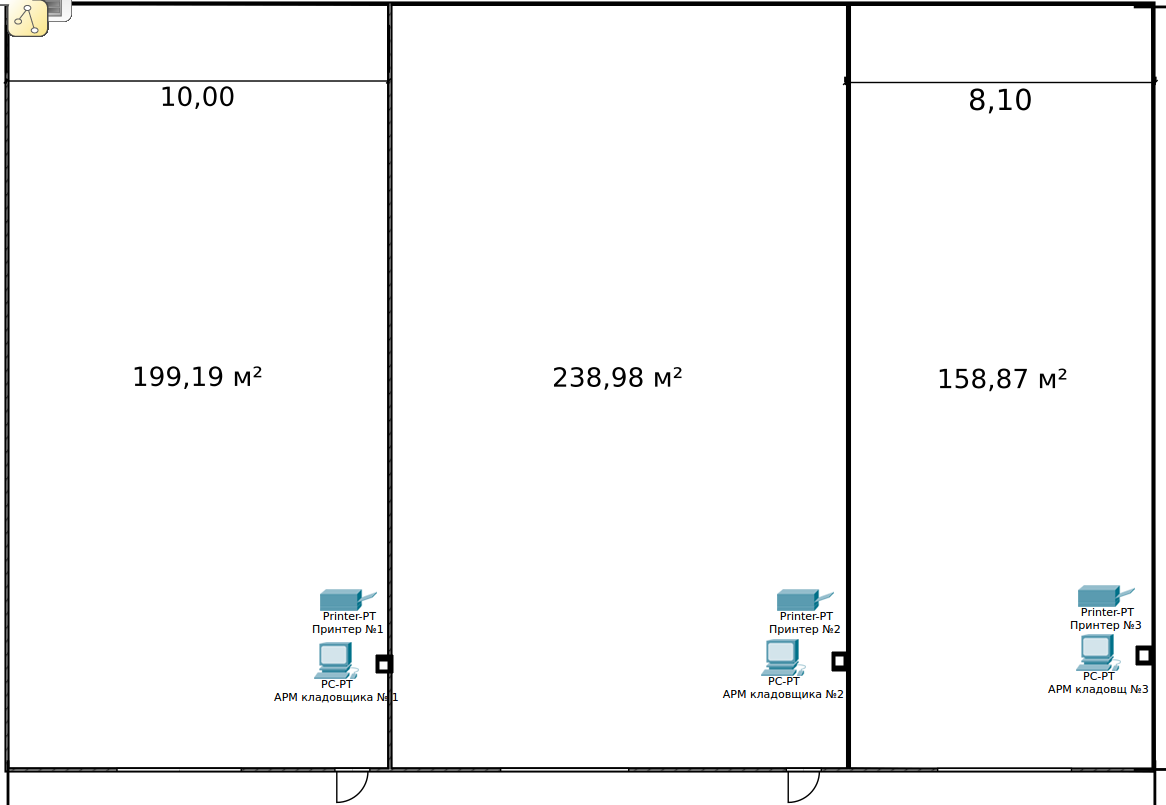
\includegraphics[width=\linewidth]{sec3/img/store.png}
  \caption{План складского здания с указанными положениями розеток и АРМ}
  \label{fig:store-arm}
\end{figure}

Сервера располaгаются в аппаратной комнате торгового здания, там же расположен телекоммуникационный шкаф, в котором размещаются коммутатор продавцов и роутер. Коммутатор кладовщиков расположен в первом помещении. Кабельная система проложена по внутренним стенам помещений на высоте 3 м от пола. Кабель, ведущий от складского до торгового здания, проложен под землей на глубине 0.5м. Расчетные длины кабелей приведены в таблице \ref{tab:cablen}.

\begin{table}[H]
  \centering
  \caption{Расчетные длины кабелей}
  \begin{tabular}{|l|l||l|l|} \hline
    Ресурс & Кабель, м & Ресурс & Кабель, м \\ \hline
    Сервер БД & 2м & АРМ продавца 1 & 1м\\ \hline
    Сервер Веб & 2м & АРМ продавца 2 & 1м \\ \hline
    Сервер бэкап & 2м & АРМ продавца 3 & 1м \\ \hline
    АРМ бухгалтера & 1м & АРМ кладовщ 1 & 1м \\ \hline
    АРМ кладовщ 3 & 1м & Принтер кладовщ 1 & 1м \\ \hline
    Принтер кладовщ 2 & 1м &АРМ кладовщ 2 & 1м \\ \hline
    Принтер кладовщ 3 & 1м& Принтер бухгалтера & 1м \\ \hline
  \end{tabular}
  \label{tab:cablen}
\end{table}

В каждом помещении имеется одна информационная розетка с двумя портами 8P8C. Розетки подключены с помощью 4-парного кабеля пятой категории (по 2 пары на порт), и прикреплены к стенам на высоте 30 см от пола.

В разрабатываемой ТКС предусмотрено 2 коммутатора. Первый коммутатор расположен в серверной торгового здания, а второй \hyp{} в помещении №1 склада. Прикреплены к стенам на высоте 3 метров. Конструкция торгового здания позволяет проводить кабель от розеток до коммутатора в стенах и потолке (т.к. перегородки гипсовые, а потолок подвесной). В складе кабели прикреплены к стенам пластиковыми хомутами. Расположение коммутаторов, роутера и прочего оборудования приведено на рисунках \ref{fig:shop-arm} и \ref{fig:store-arm}. Расчетные длины кабелей от розеток до коммутаторов приведены в таблице \ref{tab:crosscablen}

\begin{table}[H]
  \centering
  \caption{Расчетные длины кабелей от розеток до кроссового оборудования}
  \begin{tabular}{|l|l||l|l|} \hline
    Ресурс & Кабель, м & Ресурс & Кабель, м \\ \hline
    АРМ продавца1 & 8.5 & АРМ Кладовщ 1 & 5.7\\ \hline
    АРМ продавца2 & 12.7 & АРМ Кладовщ 2 & 28.7\\ \hline
    АРМ продавца3 & 25.7 & АРМ Кладовщ 3 & 35.5\\ \hline
    АРМ бухгалтера & 3.2 & & \\ \hline
  \end{tabular}
  \label{tab:crosscablen}
\end{table}

Разработанная физическая модель кабельной подсистемы локальной телекоммуникационной системы для торгового и складского зданий приведена на рисунках \ref{fig:cisco-shop} и \ref{fig:cisco-store} соответственно.

\begin{figure}[H]
  \centering
  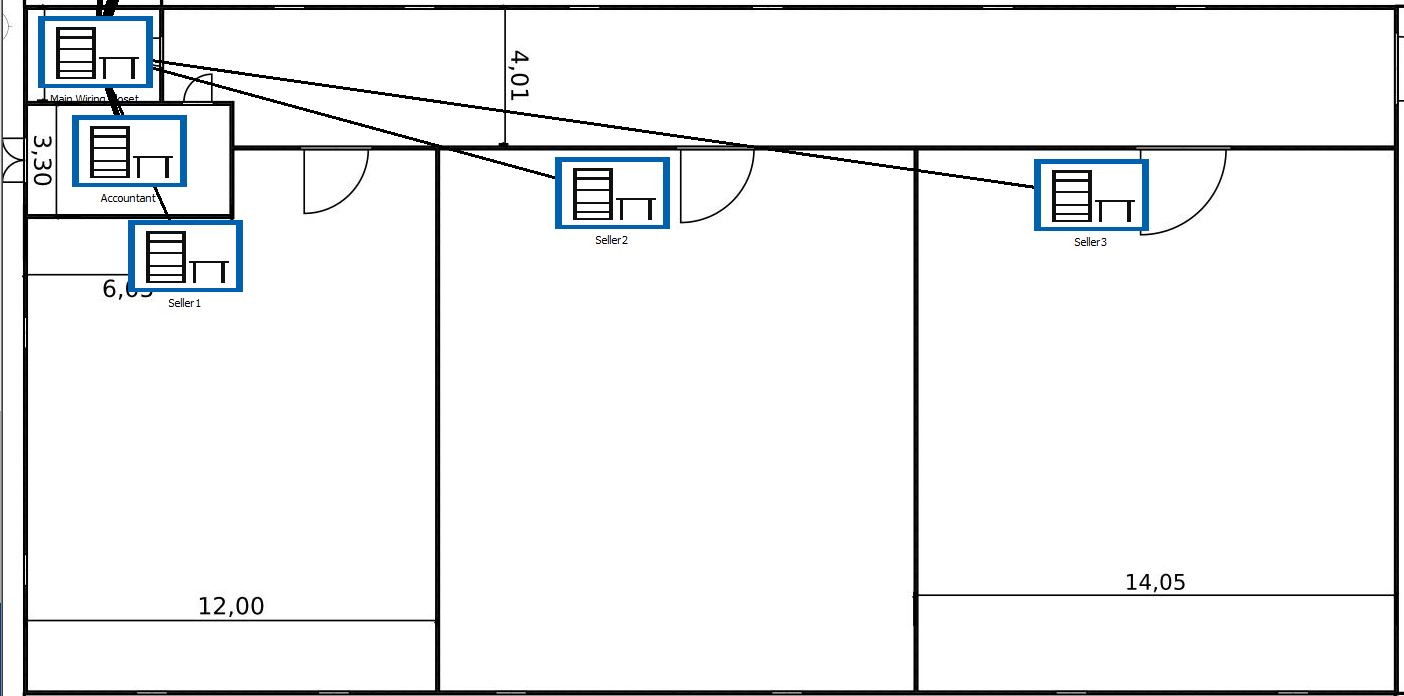
\includegraphics[width=\linewidth]{sec3/img/cisco-shop.png}
  \caption{Физическая модель кабельной подсистемы торгового здания}
  \label{fig:cisco-shop}
\end{figure}

\begin{figure}[H]
  \centering
  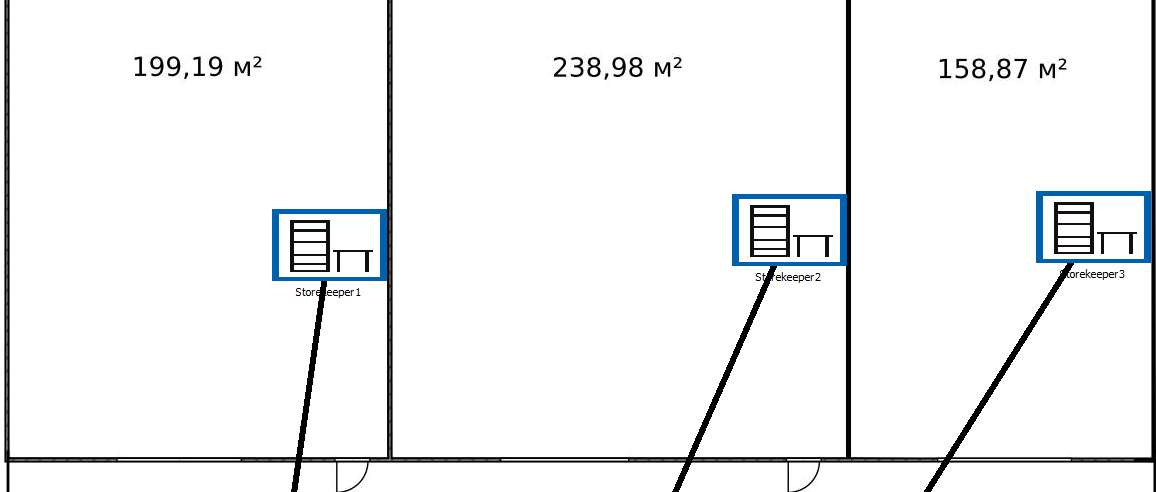
\includegraphics[width=\linewidth]{sec3/img/cisco-store.png}
  \caption{Физическая модель кабельной подсистемы складского здания}
  \label{fig:cisco-store}
\end{figure}


Для подключения к сети интернет необходим роутер с возможностью подключения оптоволоконных кабелей. Роутер, через который осуществляется подключение к интернету, расположен серверной комнате торгового здания.
% \section{Разработка модели адресации ТКС торгового склада}
\label{sec:4}
Одним из этапов разработки телекоммуникационной системы является разработка модели адресации. Данная модель приведена в таблице \ref{tab:model}.

\begin{table}[H]
  \centering
  \caption{Модель адресации телекоммуникационной системы торгового склада}
  \begin{tabular}{|c|c|c|c|} \hline
    Рабочее место & IP адрес/маска & Адрес маршрутизатора & Наименование рабочего места \\ \hline
    АРМ бухгалтера & 192.168.2.2/24 & 192.168.2.1 & АРМ Б \\ \hline
    Принтер бухгалтера & 192.168.2.22/24 & 192.168.2.1 & Пр Б \\ \hline
    АРМ Продавца 1 & 192.168.0.2/24 & 192.168.0.1 & АРМ П1 \\ \hline
    АРМ Продавца 2 & 192.168.0.3/24 & 192.168.0.1 & АРМ П2 \\ \hline
    АРМ Продавца 3 & 192.168.0.4/24 & 192.168.0.1 & АРМ П3 \\ \hline
    АРМ Кладовщ 1 & 192.168.1.2/24 & 192.168.1.1 & АРМ К1 \\ \hline
    Принтер Кладовщ 1 & 192.168.1.22/24 & 192.168.1.1 & Пр К1 \\ \hline
    АРМ Кладовщ 2 & 192.168.1.3/24 & 192.168.1.1 & АРМ К2 \\ \hline
    Принтер Кладовщ 2 & 192.168.1.33/24 & 192.168.1.1 & Пр К2 \\ \hline
    АРМ Кладовщ 3 & 192.168.1.4/24 & 192.168.1.1 & АРМ К3 \\ \hline
    Принтер Кладовщ 3 & 192.168.1.44/24 & 192.168.1.1 & Пр К3 \\ \hline
  \end{tabular}
  \label{tab:model}
\end{table}

% \section{Стоимостная оценка проекта телекоммуникационной системы торгового склада}
\label{sec:5}

На основании разработанной физической модели осуществлена стоимостная оценка проекта локальной ТКС. Оценена общая стоимость сетевого оборудования, кабелей, телекоммуникационных шкафов, серверов, МФУ, рабочих машин. Составлено 3 стоимостных оценки (верхняя, средняя, нижняя) для компонентов ТКС. Таблицы с верхней, средней и нижней оценками приведены в таблицах \ref{tab:est}, \ref{tab:estm}, \ref{tab:ests}.

\begin{table}[H]
  \centering
  \caption{Оценка стоимости компонентов ТКС}
  \begin{tabular}{|p{7cm}|l|l|l|} \hline
    Наименование компонента & Количество, ед. & Цена, руб.& Стоимость, руб \\ \hline
    Коммутатор Cisco SLM2008T & 3 & 7646 & 22938 \\ \hline
    Маршрутизатор D-link DSR-250 & 1 & 10850 & 10850 \\ \hline
    Серверная платформа ASUS RS700D-E6/PS8 & 2 & 121355 & 242710 \\ \hline
    Внешний жесткий диск 8Tb Seagate STCS8000201 Personal Cloud 2-Bay NAS
(сетевое хранилище) & 1 & 32750 & 32750 \\ \hline
    Ноутбук Lenovo IdeaPad B5010G & 7 & 19390 & 135730 \\ \hline
    МФУ CANON i-SENSYS MF212w & 7 & 8660 & 60620 \\ \hline
    Шкаф серверный Lanmaster Business (TWT-CBB-42U-6X10-00) 19U & 1 & 47920 & 47920 \\ \hline
    Розетка компьютерная RJ-45(8P8C), категория 5, двойная, внешняя & 7 & 160 & 1120 \\ \hline
    Кабель BC5E-4-OP для внешней прокладки , неэкранированный & 30 м & 71 & 2130 \\ \hline
    Кабель UTP 4 Pairs Cat 5 & 138 м & 13 & 1794 \\ \hline
    Лоток кабельный перфорированный & 35м & 170 & 5950 \\ \hline
    Защитная труба Oventrop & 25м & 130 & 3250 \\ \hline
    & & Итого & 558762 \\ \hline
  \end{tabular}
  \label{tab:est}
\end{table}

\begin{table}[H]
  \centering
  \caption{Средняя оценка стоимости компонентов ТКС}
  \begin{tabular}{|p{7cm}|l|l|l|} \hline
    Наименование компонента & Количество, ед. & Цена, руб.& Стоимость, руб \\ \hline
    Коммутатор Cisco SLM2008T & 3 & 7646 & 22938 \\ \hline
    Маршрутизатор D-link DFL-260E & 1 & 10850 & 10850 \\ \hline
    Lenovo Erazer X310 & 2 & 90840 & 181680 \\ \hline
    Внешний жесткий диск 8Tb Seagate STCS8000201 Personal Cloud 2-Bay NAS
(сетевое хранилище) & 1 & 32750 & 32750 \\ \hline
    Ноутбук IRU D1001 & 7 & 12590 & 88130 \\ \hline
    МФУ CANON i-SENSYS MF212w & 7 & 8660 & 60620 \\ \hline
    Шкаф серверный Lanmaster Business (TWT-CBB-42U-6X10-00) 19U & 1 & 25800 & 25800 \\ \hline
    Розетка компьютерная RJ-45(8P8C), категория 5, двойная, внешняя & 7 & 160 & 1120 \\ \hline
    Кабель BC5E-4-OP для внешней прокладки , неэкранированный & 30 м & 71 & 2130 \\ \hline
    Кабель UTP 4 Pairs Cat 5 & 138 м & 13 & 1794 \\ \hline
    Лоток кабельный перфорированный & 35м & 170 & 5950 \\ \hline
    Защитная труба Oventrop & 25м & 130 & 3250 \\ \hline
    & & Итого & 437012 \\ \hline
  \end{tabular}
  \label{tab:estm}
\end{table}

\begin{table}[H]
  \centering
  \caption{Нижняя оценка стоимости компонентов ТКС}
  \begin{tabular}{|p{7cm}|l|l|l|} \hline
    Наименование компонента & Количество, ед. & Цена, руб.& Стоимость, руб \\ \hline
    Коммутатор TP-LINK TL-SG1008D & 3 & 1550 & 4650 \\ \hline
    Маршрутизатор TP-LINK Archer C2 & 1 & 3000 & 3000 \\ \hline
    Lenovo Erazer X310 & 2 & 90840 & 181680 \\ \hline
    Внешний жесткий диск 2Tb Seagate STCS2000201 Personal Cloud 2-Bay NAS
(сетевое хранилище) & 1 & 13540 & 13540 \\ \hline
    Ноутбук IRU D1001 & 7 & 12590 & 88130 \\ \hline
    МФУ CANON i-SENSYS MF212w & 7 & 8660 & 60620 \\ \hline
    Шкаф серверный Lanmaster Business (TWT-CBB-42U-6X10-00) 19U & 1 & 25800 & 25800 \\ \hline
    Розетка компьютерная RJ-45(8P8C), категория 5, двойная, внешняя & 7 & 160 & 1120 \\ \hline
    Кабель BC5E-4-OP для внешней прокладки , неэкранированный & 30 м & 71 & 2130 \\ \hline
    Кабель UTP 4 Pairs Cat 5 & 138 м & 13 & 1794 \\ \hline
    Лоток кабельный перфорированный & 35м & 170 & 5950 \\ \hline
    Защитная труба Oventrop & 25м & 130 & 3250 \\ \hline
    & & Итого & 391664 \\ \hline
  \end{tabular}
  \label{tab:ests}
\end{table}

На основании проведенной стоимостной оценки и анализа выполняемых функций ТКС было принято решение о покупке элементов, относящихся к средней оценке стоимости.
\specsection{Заключение}

В данной работе разработан проект локальной телекоммуникационной системы торгового склада. 

В ходе выполнения работы разработаны инфологическая и структурная модели информационной системы организации, сформулированы и описаны цели использования сети и её отдельных составляющих компонентов. Выбраны и обоснованы размеры и структура сети, выбрана кабельная подсистема сети, оценены основные характеристики и размеры кабельной системы. 

Выбрано сетевое оборудование. Присвоены адреса основным элементам сети. Выполнено моделирование структурной схемы локальной телекоммуникационной системы в среде Packet Tracer и стоимостная оценка принятых решений.

В результате работы закреплены и углублены знания по организации локальной телекоммуникационной системы и выработаны практические навыки. 

Таким образом, адание на курсовое проектирование выполнено в полном объёме.  
\specsection{Список использованных источников}

1 В. А. Мали, О. В. Липилин. Проектирование ЛТКС. Пенза, Изд. ПГУ,  2015.
%\anonsection{Приложение 1}
\label{app:1}
\begin{sidewaysfigure}[H]
    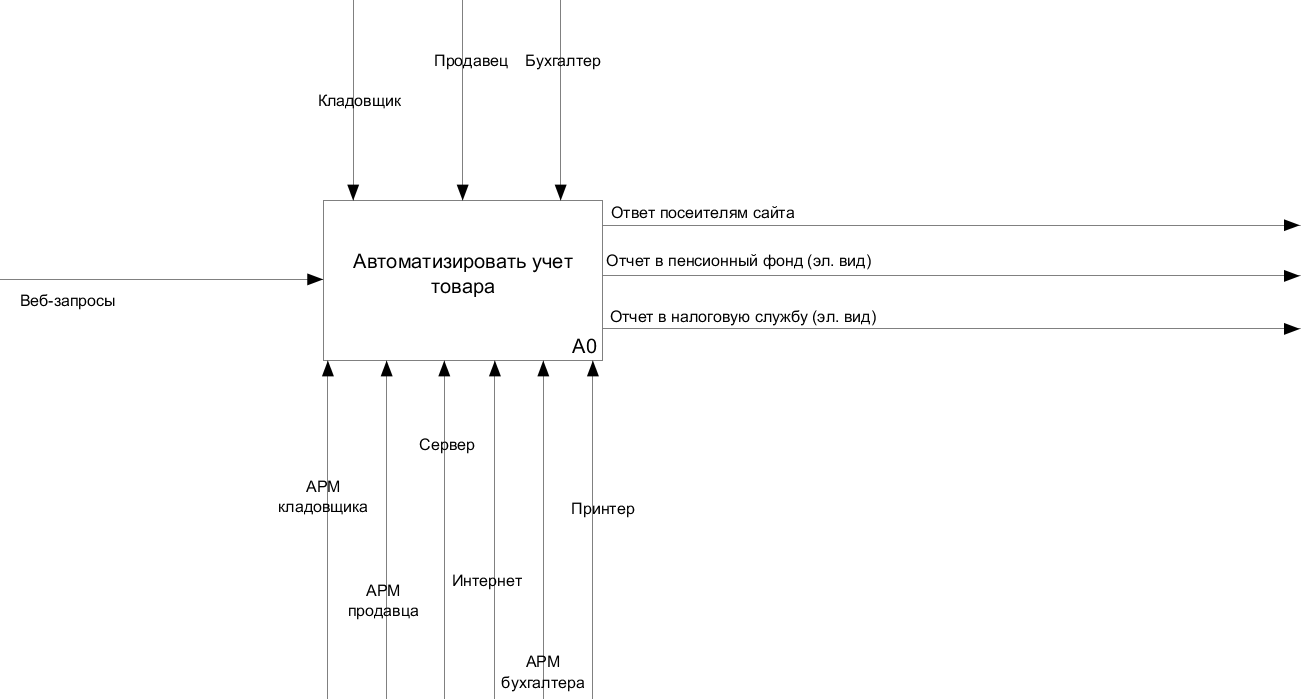
\includegraphics{appendix/a0.png}
    \caption{Целевая функция телекоммуникационной системы торгового склада}
    \label{fig:idef0-common}
\end{sidewaysfigure}
\newpage
\appsection{Название приложения}{prove}
Само приложение 1.
\newpage
\begin{equation}
  \label{eq:3}
  y = sin(x)
\end{equation}

\begin{equation}
  \label{eq:4}
  y = sin(x)
\end{equation}
\appsection{Название приложения2}{prove2}
Само приложение 2. skdfh sjdlf hsldf jsdhf sljfh sdfjl sdljf sdlfjshdf ls dhfjsdhf jshf lsjd sjdhf lsdhjf sljdf shjf lsjhdf sljdf sjdf shdfls dfhsdjf 


%Длинная таблица
\setlength\LTleft{0pt}
\setlength\LTright{0pt}
\begin{longtable}{|@{\extracolsep{\fill}} r|*{2}{l|}}
\caption{Feasible triples for 
highly variable Grid, MLMMH} \label{grid_mlmmh}\\
%\multicolumn{колво колонок}{|l|c|r|}{текст}
%добавлять и удалять только multicolumn
\hline \multicolumn{1}{|p{1cm}|}{Time (s)} & % Колонки таблицы в 
\multicolumn{1}{c|}{Triple chosen} & % первой части таблицы
\multicolumn{1}{c|}{Other feasible triples} \\
\hline 
\endfirsthead
\captionsetup{labelformat=continued} %%Продолжение
\caption[]{}\\ %%таблицы (caption)
\hline 
\multicolumn{1}{|p{1cm}|}{Time (s)} & %Заговолки в продолжении
\multicolumn{1}{c|}{Triple chosen} & % Те же самые
\multicolumn{1}{c|}{Other feasible triples} \\ 
\hline 
\endhead
\hline
\endfoot
\hline
\endlastfoot

0 & (1, 11, 13725) & (1, 12, 10980), (1, 13, 8235), (2, 2, 0), (3, 1, 0) \\
2745 & (1, 12, 10980) & (1, 13, 8235), (2, 2, 0), (2, 3, 0), (3, 1, 0) \\
5490 & (1, 12, 13725) & (2, 2, 2745), (2, 3, 0), (3, 1, 0) \\
8235 & (1, 12, 16470) & (1, 13, 13725), (2, 2, 2745), (2, 3, 0), (3, 1, 0) \\
10980 & (1, 12, 16470) & (1, 13, 13725), (2, 2, 2745), (2, 3, 0), (3, 1, 0) \\
13725 & (1, 12, 16470) & (1, 13, 13725), (2, 2, 2745), (2, 3, 0), (3, 1, 0) \\
16470 & (1, 13, 16470) & (2, 2, 2745), (2, 3, 0), (3, 1, 0) \\
19215 & (1, 12, 16470) & (1, 13, 13725), (2, 2, 2745), (2, 3, 0), (3, 1, 0) \\
21960 & (1, 12, 16470) & (1, 13, 13725), (2, 2, 2745), (2, 3, 0), (3, 1, 0) \\
24705 & (1, 12, 16470) & (1, 13, 13725), (2, 2, 2745), (2, 3, 0), (3, 1, 0) \\
27450 & (1, 12, 16470) & (1, 13, 13725), (2, 2, 2745), (2, 3, 0), (3, 1, 0) \\
30195 & (2, 2, 2745) & (2, 3, 0), (3, 1, 0) \\
32940 & (1, 13, 16470) & (2, 2, 2745), (2, 3, 0), (3, 1, 0) \\
35685 & (1, 13, 13725) & (2, 2, 2745), (2, 3, 0), (3, 1, 0) \\
38430 & (1, 13, 10980) & (2, 2, 2745), (2, 3, 0), (3, 1, 0) \\
\end{longtable}

\begin{equation}
  \label{eq:1}
  x = \sin(x)
\end{equation}

\begin{equation}
  x = \sin(x)
\end{equation}

\begin{equation}
  \label{eq:2}
  x = \sin(x)
\end{equation}

\newpage
\begin{lstlisting}[caption={Быдлокод}, captionpos=b]
#include <iostream>
using namespace std;
int main()
{
  char x[] = "aoeuu";
  int i = 0;
  while(x[i] != '\0')
    i++;
  
  return 0;
}
\end{lstlisting}

\end{document}
